% Created by tikzDevice version 0.12.6 on 2024-03-24 19:09:25
% !TEX encoding = UTF-8 Unicode
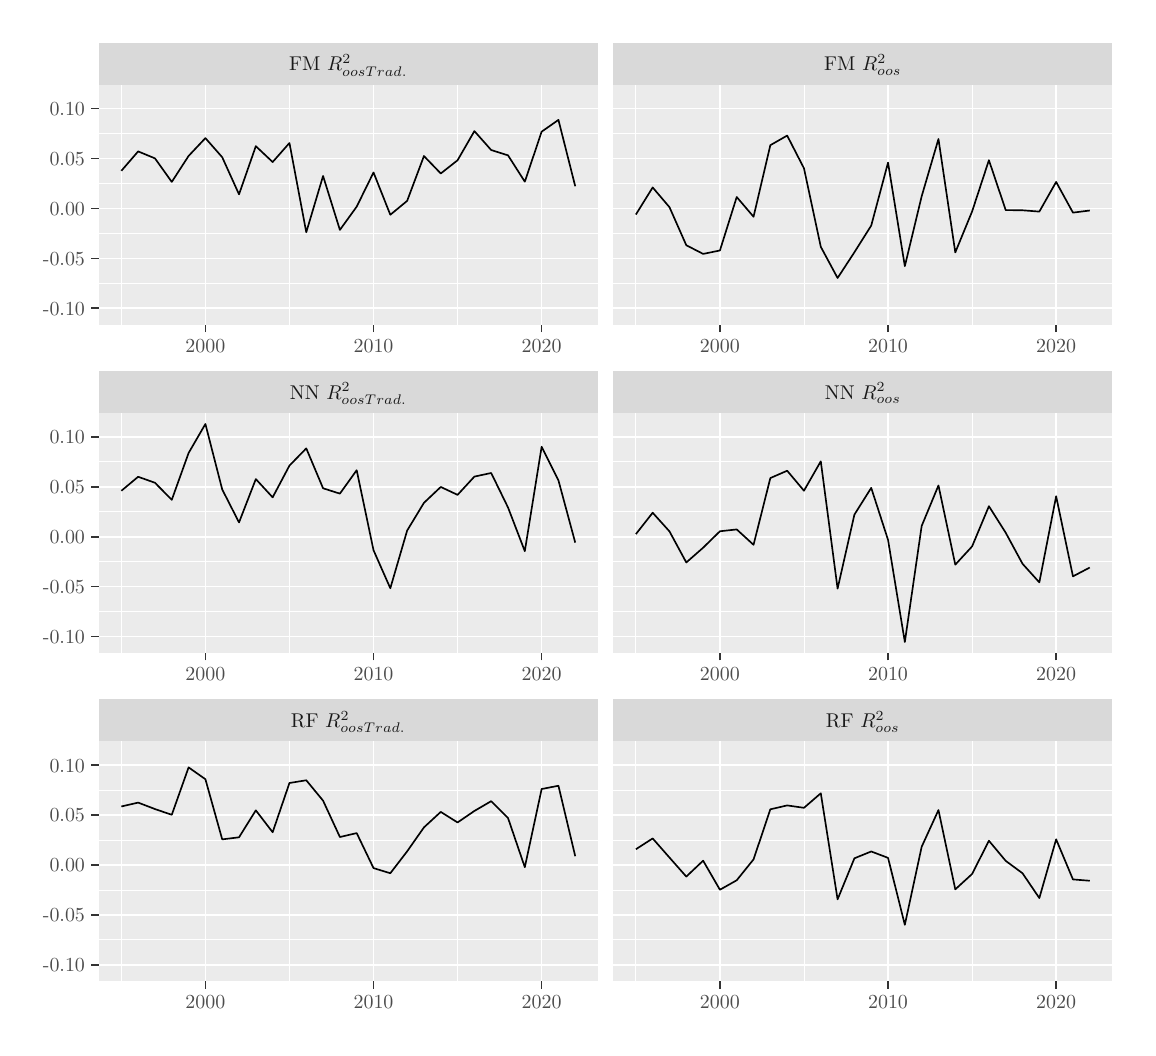
\begin{tikzpicture}[x=1pt,y=1pt]
\definecolor{fillColor}{RGB}{255,255,255}
\path[use as bounding box,fill=fillColor,fill opacity=0.00] (0,0) rectangle (397.48,361.35);
\begin{scope}
\path[clip] (  0.00,  0.00) rectangle (397.48,361.35);
\definecolor{drawColor}{RGB}{255,255,255}
\definecolor{fillColor}{RGB}{255,255,255}

\path[draw=drawColor,line width= 0.6pt,line join=round,line cap=round,fill=fillColor] (  0.00,  0.00) rectangle (397.48,361.35);
\end{scope}
\begin{scope}
\path[clip] ( 25.65,254.04) rectangle (206.07,340.69);
\definecolor{fillColor}{gray}{0.92}

\path[fill=fillColor] ( 25.65,254.04) rectangle (206.07,340.69);
\definecolor{drawColor}{RGB}{255,255,255}

\path[draw=drawColor,line width= 0.3pt,line join=round] ( 25.65,268.97) --
	(206.07,268.97);

\path[draw=drawColor,line width= 0.3pt,line join=round] ( 25.65,287.00) --
	(206.07,287.00);

\path[draw=drawColor,line width= 0.3pt,line join=round] ( 25.65,305.03) --
	(206.07,305.03);

\path[draw=drawColor,line width= 0.3pt,line join=round] ( 25.65,323.07) --
	(206.07,323.07);

\path[draw=drawColor,line width= 0.3pt,line join=round] ( 33.85,254.04) --
	( 33.85,340.69);

\path[draw=drawColor,line width= 0.3pt,line join=round] ( 94.59,254.04) --
	( 94.59,340.69);

\path[draw=drawColor,line width= 0.3pt,line join=round] (155.34,254.04) --
	(155.34,340.69);

\path[draw=drawColor,line width= 0.6pt,line join=round] ( 25.65,259.95) --
	(206.07,259.95);

\path[draw=drawColor,line width= 0.6pt,line join=round] ( 25.65,277.98) --
	(206.07,277.98);

\path[draw=drawColor,line width= 0.6pt,line join=round] ( 25.65,296.02) --
	(206.07,296.02);

\path[draw=drawColor,line width= 0.6pt,line join=round] ( 25.65,314.05) --
	(206.07,314.05);

\path[draw=drawColor,line width= 0.6pt,line join=round] ( 25.65,332.08) --
	(206.07,332.08);

\path[draw=drawColor,line width= 0.6pt,line join=round] ( 64.22,254.04) --
	( 64.22,340.69);

\path[draw=drawColor,line width= 0.6pt,line join=round] (124.97,254.04) --
	(124.97,340.69);

\path[draw=drawColor,line width= 0.6pt,line join=round] (185.72,254.04) --
	(185.72,340.69);
\definecolor{drawColor}{RGB}{0,0,0}

\path[draw=drawColor,line width= 0.6pt,line join=round] ( 33.85,309.62) --
	( 39.92,316.64) --
	( 46.00,314.12) --
	( 52.07,305.61) --
	( 58.15,315.00) --
	( 64.22,321.44) --
	( 70.30,314.53) --
	( 76.37,301.12) --
	( 82.44,318.52) --
	( 88.52,312.80) --
	( 94.59,319.67) --
	(100.67,287.42) --
	(106.74,307.76) --
	(112.82,288.27) --
	(118.89,296.67) --
	(124.97,309.02) --
	(131.04,293.74) --
	(137.12,298.76) --
	(143.19,314.96) --
	(149.27,308.66) --
	(155.34,313.43) --
	(161.42,323.97) --
	(167.49,317.13) --
	(173.57,315.21) --
	(179.64,305.70) --
	(185.72,323.76) --
	(191.79,328.02) --
	(197.86,304.04);
\end{scope}
\begin{scope}
\path[clip] ( 25.65,135.43) rectangle (206.07,222.07);
\definecolor{fillColor}{gray}{0.92}

\path[fill=fillColor] ( 25.65,135.43) rectangle (206.07,222.07);
\definecolor{drawColor}{RGB}{255,255,255}

\path[draw=drawColor,line width= 0.3pt,line join=round] ( 25.65,150.35) --
	(206.07,150.35);

\path[draw=drawColor,line width= 0.3pt,line join=round] ( 25.65,168.38) --
	(206.07,168.38);

\path[draw=drawColor,line width= 0.3pt,line join=round] ( 25.65,186.42) --
	(206.07,186.42);

\path[draw=drawColor,line width= 0.3pt,line join=round] ( 25.65,204.45) --
	(206.07,204.45);

\path[draw=drawColor,line width= 0.3pt,line join=round] ( 33.85,135.43) --
	( 33.85,222.07);

\path[draw=drawColor,line width= 0.3pt,line join=round] ( 94.59,135.43) --
	( 94.59,222.07);

\path[draw=drawColor,line width= 0.3pt,line join=round] (155.34,135.43) --
	(155.34,222.07);

\path[draw=drawColor,line width= 0.6pt,line join=round] ( 25.65,141.33) --
	(206.07,141.33);

\path[draw=drawColor,line width= 0.6pt,line join=round] ( 25.65,159.37) --
	(206.07,159.37);

\path[draw=drawColor,line width= 0.6pt,line join=round] ( 25.65,177.40) --
	(206.07,177.40);

\path[draw=drawColor,line width= 0.6pt,line join=round] ( 25.65,195.43) --
	(206.07,195.43);

\path[draw=drawColor,line width= 0.6pt,line join=round] ( 25.65,213.47) --
	(206.07,213.47);

\path[draw=drawColor,line width= 0.6pt,line join=round] ( 64.22,135.43) --
	( 64.22,222.07);

\path[draw=drawColor,line width= 0.6pt,line join=round] (124.97,135.43) --
	(124.97,222.07);

\path[draw=drawColor,line width= 0.6pt,line join=round] (185.72,135.43) --
	(185.72,222.07);
\definecolor{drawColor}{RGB}{0,0,0}

\path[draw=drawColor,line width= 0.6pt,line join=round] ( 33.85,194.00) --
	( 39.92,199.06) --
	( 46.00,196.90) --
	( 52.07,190.73) --
	( 58.15,207.66) --
	( 64.22,218.14) --
	( 70.30,194.48) --
	( 76.37,182.57) --
	( 82.44,198.23) --
	( 88.52,191.63) --
	( 94.59,203.10) --
	(100.67,209.33) --
	(106.74,194.91) --
	(112.82,192.97) --
	(118.89,201.44) --
	(124.97,172.52) --
	(131.04,158.78) --
	(137.12,179.63) --
	(143.19,189.65) --
	(149.27,195.39) --
	(155.34,192.53) --
	(161.42,199.13) --
	(167.49,200.43) --
	(173.57,187.97) --
	(179.64,172.18) --
	(185.72,209.93) --
	(191.79,197.77) --
	(197.86,175.27);
\end{scope}
\begin{scope}
\path[clip] ( 25.65, 16.81) rectangle (206.07,103.46);
\definecolor{fillColor}{gray}{0.92}

\path[fill=fillColor] ( 25.65, 16.81) rectangle (206.07,103.46);
\definecolor{drawColor}{RGB}{255,255,255}

\path[draw=drawColor,line width= 0.3pt,line join=round] ( 25.65, 31.73) --
	(206.07, 31.73);

\path[draw=drawColor,line width= 0.3pt,line join=round] ( 25.65, 49.77) --
	(206.07, 49.77);

\path[draw=drawColor,line width= 0.3pt,line join=round] ( 25.65, 67.80) --
	(206.07, 67.80);

\path[draw=drawColor,line width= 0.3pt,line join=round] ( 25.65, 85.83) --
	(206.07, 85.83);

\path[draw=drawColor,line width= 0.3pt,line join=round] ( 33.85, 16.81) --
	( 33.85,103.46);

\path[draw=drawColor,line width= 0.3pt,line join=round] ( 94.59, 16.81) --
	( 94.59,103.46);

\path[draw=drawColor,line width= 0.3pt,line join=round] (155.34, 16.81) --
	(155.34,103.46);

\path[draw=drawColor,line width= 0.6pt,line join=round] ( 25.65, 22.72) --
	(206.07, 22.72);

\path[draw=drawColor,line width= 0.6pt,line join=round] ( 25.65, 40.75) --
	(206.07, 40.75);

\path[draw=drawColor,line width= 0.6pt,line join=round] ( 25.65, 58.78) --
	(206.07, 58.78);

\path[draw=drawColor,line width= 0.6pt,line join=round] ( 25.65, 76.82) --
	(206.07, 76.82);

\path[draw=drawColor,line width= 0.6pt,line join=round] ( 25.65, 94.85) --
	(206.07, 94.85);

\path[draw=drawColor,line width= 0.6pt,line join=round] ( 64.22, 16.81) --
	( 64.22,103.46);

\path[draw=drawColor,line width= 0.6pt,line join=round] (124.97, 16.81) --
	(124.97,103.46);

\path[draw=drawColor,line width= 0.6pt,line join=round] (185.72, 16.81) --
	(185.72,103.46);
\definecolor{drawColor}{RGB}{0,0,0}

\path[draw=drawColor,line width= 0.6pt,line join=round] ( 33.85, 79.93) --
	( 39.92, 81.33) --
	( 46.00, 79.00) --
	( 52.07, 76.92) --
	( 58.15, 94.05) --
	( 64.22, 89.78) --
	( 70.30, 68.04) --
	( 76.37, 68.79) --
	( 82.44, 78.53) --
	( 88.52, 70.62) --
	( 94.59, 88.41) --
	(100.67, 89.40) --
	(106.74, 82.03) --
	(112.82, 68.89) --
	(118.89, 70.31) --
	(124.97, 57.66) --
	(131.04, 55.80) --
	(137.12, 63.71) --
	(143.19, 72.37) --
	(149.27, 77.97) --
	(155.34, 74.15) --
	(161.42, 78.31) --
	(167.49, 81.85) --
	(173.57, 75.76) --
	(179.64, 57.98) --
	(185.72, 86.24) --
	(191.79, 87.42) --
	(197.86, 61.96);
\end{scope}
\begin{scope}
\path[clip] (211.57,254.04) rectangle (391.98,340.69);
\definecolor{fillColor}{gray}{0.92}

\path[fill=fillColor] (211.57,254.04) rectangle (391.98,340.69);
\definecolor{drawColor}{RGB}{255,255,255}

\path[draw=drawColor,line width= 0.3pt,line join=round] (211.57,268.97) --
	(391.98,268.97);

\path[draw=drawColor,line width= 0.3pt,line join=round] (211.57,287.00) --
	(391.98,287.00);

\path[draw=drawColor,line width= 0.3pt,line join=round] (211.57,305.03) --
	(391.98,305.03);

\path[draw=drawColor,line width= 0.3pt,line join=round] (211.57,323.07) --
	(391.98,323.07);

\path[draw=drawColor,line width= 0.3pt,line join=round] (219.77,254.04) --
	(219.77,340.69);

\path[draw=drawColor,line width= 0.3pt,line join=round] (280.51,254.04) --
	(280.51,340.69);

\path[draw=drawColor,line width= 0.3pt,line join=round] (341.26,254.04) --
	(341.26,340.69);

\path[draw=drawColor,line width= 0.6pt,line join=round] (211.57,259.95) --
	(391.98,259.95);

\path[draw=drawColor,line width= 0.6pt,line join=round] (211.57,277.98) --
	(391.98,277.98);

\path[draw=drawColor,line width= 0.6pt,line join=round] (211.57,296.02) --
	(391.98,296.02);

\path[draw=drawColor,line width= 0.6pt,line join=round] (211.57,314.05) --
	(391.98,314.05);

\path[draw=drawColor,line width= 0.6pt,line join=round] (211.57,332.08) --
	(391.98,332.08);

\path[draw=drawColor,line width= 0.6pt,line join=round] (250.14,254.04) --
	(250.14,340.69);

\path[draw=drawColor,line width= 0.6pt,line join=round] (310.89,254.04) --
	(310.89,340.69);

\path[draw=drawColor,line width= 0.6pt,line join=round] (371.63,254.04) --
	(371.63,340.69);
\definecolor{drawColor}{RGB}{0,0,0}

\path[draw=drawColor,line width= 0.6pt,line join=round] (219.77,293.82) --
	(225.84,303.61) --
	(231.92,296.47) --
	(237.99,282.73) --
	(244.07,279.60) --
	(250.14,280.83) --
	(256.21,300.15) --
	(262.29,293.03) --
	(268.36,318.88) --
	(274.44,322.35) --
	(280.51,310.54) --
	(286.59,282.16) --
	(292.66,270.89) --
	(298.74,280.20) --
	(304.81,289.83) --
	(310.89,312.58) --
	(316.96,275.16) --
	(323.04,300.41) --
	(329.11,321.12) --
	(335.19,280.14) --
	(341.26,294.92) --
	(347.34,313.46) --
	(353.41,295.43) --
	(359.49,295.36) --
	(365.56,294.88) --
	(371.63,305.60) --
	(377.71,294.51) --
	(383.78,295.28);
\end{scope}
\begin{scope}
\path[clip] (211.57,135.43) rectangle (391.98,222.07);
\definecolor{fillColor}{gray}{0.92}

\path[fill=fillColor] (211.57,135.43) rectangle (391.98,222.07);
\definecolor{drawColor}{RGB}{255,255,255}

\path[draw=drawColor,line width= 0.3pt,line join=round] (211.57,150.35) --
	(391.98,150.35);

\path[draw=drawColor,line width= 0.3pt,line join=round] (211.57,168.38) --
	(391.98,168.38);

\path[draw=drawColor,line width= 0.3pt,line join=round] (211.57,186.42) --
	(391.98,186.42);

\path[draw=drawColor,line width= 0.3pt,line join=round] (211.57,204.45) --
	(391.98,204.45);

\path[draw=drawColor,line width= 0.3pt,line join=round] (219.77,135.43) --
	(219.77,222.07);

\path[draw=drawColor,line width= 0.3pt,line join=round] (280.51,135.43) --
	(280.51,222.07);

\path[draw=drawColor,line width= 0.3pt,line join=round] (341.26,135.43) --
	(341.26,222.07);

\path[draw=drawColor,line width= 0.6pt,line join=round] (211.57,141.33) --
	(391.98,141.33);

\path[draw=drawColor,line width= 0.6pt,line join=round] (211.57,159.37) --
	(391.98,159.37);

\path[draw=drawColor,line width= 0.6pt,line join=round] (211.57,177.40) --
	(391.98,177.40);

\path[draw=drawColor,line width= 0.6pt,line join=round] (211.57,195.43) --
	(391.98,195.43);

\path[draw=drawColor,line width= 0.6pt,line join=round] (211.57,213.47) --
	(391.98,213.47);

\path[draw=drawColor,line width= 0.6pt,line join=round] (250.14,135.43) --
	(250.14,222.07);

\path[draw=drawColor,line width= 0.6pt,line join=round] (310.89,135.43) --
	(310.89,222.07);

\path[draw=drawColor,line width= 0.6pt,line join=round] (371.63,135.43) --
	(371.63,222.07);
\definecolor{drawColor}{RGB}{0,0,0}

\path[draw=drawColor,line width= 0.6pt,line join=round] (219.77,178.34) --
	(225.84,186.07) --
	(231.92,179.32) --
	(237.99,168.10) --
	(244.07,173.43) --
	(250.14,179.37) --
	(256.21,180.04) --
	(262.29,174.48) --
	(268.36,198.60) --
	(274.44,201.25) --
	(280.51,194.03) --
	(286.59,204.65) --
	(292.66,158.64) --
	(298.74,185.40) --
	(304.81,195.05) --
	(310.89,176.26) --
	(316.96,139.36) --
	(323.04,181.28) --
	(329.11,195.93) --
	(335.19,167.31) --
	(341.26,173.90) --
	(347.34,188.43) --
	(353.41,178.84) --
	(359.49,167.62) --
	(365.56,160.90) --
	(371.63,192.03) --
	(377.71,163.08) --
	(383.78,166.27);
\end{scope}
\begin{scope}
\path[clip] (211.57, 16.81) rectangle (391.98,103.46);
\definecolor{fillColor}{gray}{0.92}

\path[fill=fillColor] (211.57, 16.81) rectangle (391.98,103.46);
\definecolor{drawColor}{RGB}{255,255,255}

\path[draw=drawColor,line width= 0.3pt,line join=round] (211.57, 31.73) --
	(391.98, 31.73);

\path[draw=drawColor,line width= 0.3pt,line join=round] (211.57, 49.77) --
	(391.98, 49.77);

\path[draw=drawColor,line width= 0.3pt,line join=round] (211.57, 67.80) --
	(391.98, 67.80);

\path[draw=drawColor,line width= 0.3pt,line join=round] (211.57, 85.83) --
	(391.98, 85.83);

\path[draw=drawColor,line width= 0.3pt,line join=round] (219.77, 16.81) --
	(219.77,103.46);

\path[draw=drawColor,line width= 0.3pt,line join=round] (280.51, 16.81) --
	(280.51,103.46);

\path[draw=drawColor,line width= 0.3pt,line join=round] (341.26, 16.81) --
	(341.26,103.46);

\path[draw=drawColor,line width= 0.6pt,line join=round] (211.57, 22.72) --
	(391.98, 22.72);

\path[draw=drawColor,line width= 0.6pt,line join=round] (211.57, 40.75) --
	(391.98, 40.75);

\path[draw=drawColor,line width= 0.6pt,line join=round] (211.57, 58.78) --
	(391.98, 58.78);

\path[draw=drawColor,line width= 0.6pt,line join=round] (211.57, 76.82) --
	(391.98, 76.82);

\path[draw=drawColor,line width= 0.6pt,line join=round] (211.57, 94.85) --
	(391.98, 94.85);

\path[draw=drawColor,line width= 0.6pt,line join=round] (250.14, 16.81) --
	(250.14,103.46);

\path[draw=drawColor,line width= 0.6pt,line join=round] (310.89, 16.81) --
	(310.89,103.46);

\path[draw=drawColor,line width= 0.6pt,line join=round] (371.63, 16.81) --
	(371.63,103.46);
\definecolor{drawColor}{RGB}{0,0,0}

\path[draw=drawColor,line width= 0.6pt,line join=round] (219.77, 64.47) --
	(225.84, 68.38) --
	(231.92, 61.46) --
	(237.99, 54.59) --
	(244.07, 60.34) --
	(250.14, 49.84) --
	(256.21, 53.26) --
	(262.29, 60.81) --
	(268.36, 78.90) --
	(274.44, 80.31) --
	(280.51, 79.44) --
	(286.59, 84.70) --
	(292.66, 46.37) --
	(298.74, 61.20) --
	(304.81, 63.67) --
	(310.89, 61.36) --
	(316.96, 37.18) --
	(323.04, 65.36) --
	(329.11, 78.63) --
	(335.19, 49.98) --
	(341.26, 55.53) --
	(347.34, 67.54) --
	(353.41, 60.28) --
	(359.49, 55.79) --
	(365.56, 46.83) --
	(371.63, 68.06) --
	(377.71, 53.57) --
	(383.78, 53.09);
\end{scope}
\begin{scope}
\path[clip] ( 25.65,103.46) rectangle (206.07,118.62);
\definecolor{fillColor}{gray}{0.85}

\path[fill=fillColor] ( 25.65,103.46) rectangle (206.07,118.62);
\definecolor{drawColor}{gray}{0.10}

\node[text=drawColor,anchor=base,inner sep=0pt, outer sep=0pt, scale=  0.72] at (115.86,108.56) {RF $R^2_{oos  Trad.}$};
\end{scope}
\begin{scope}
\path[clip] (211.57,103.46) rectangle (391.98,118.62);
\definecolor{fillColor}{gray}{0.85}

\path[fill=fillColor] (211.57,103.46) rectangle (391.98,118.62);
\definecolor{drawColor}{gray}{0.10}

\node[text=drawColor,anchor=base,inner sep=0pt, outer sep=0pt, scale=  0.72] at (301.78,108.56) {RF $R^2_{oos}$};
\end{scope}
\begin{scope}
\path[clip] ( 25.65,222.07) rectangle (206.07,237.23);
\definecolor{fillColor}{gray}{0.85}

\path[fill=fillColor] ( 25.65,222.07) rectangle (206.07,237.23);
\definecolor{drawColor}{gray}{0.10}

\node[text=drawColor,anchor=base,inner sep=0pt, outer sep=0pt, scale=  0.72] at (115.86,227.17) {NN $R^2_{oos  Trad.}$};
\end{scope}
\begin{scope}
\path[clip] (211.57,222.07) rectangle (391.98,237.23);
\definecolor{fillColor}{gray}{0.85}

\path[fill=fillColor] (211.57,222.07) rectangle (391.98,237.23);
\definecolor{drawColor}{gray}{0.10}

\node[text=drawColor,anchor=base,inner sep=0pt, outer sep=0pt, scale=  0.72] at (301.78,227.17) {NN $R^2_{oos}$};
\end{scope}
\begin{scope}
\path[clip] ( 25.65,340.69) rectangle (206.07,355.85);
\definecolor{fillColor}{gray}{0.85}

\path[fill=fillColor] ( 25.65,340.69) rectangle (206.07,355.85);
\definecolor{drawColor}{gray}{0.10}

\node[text=drawColor,anchor=base,inner sep=0pt, outer sep=0pt, scale=  0.72] at (115.86,345.79) {FM $R^2_{oos  Trad.}$};
\end{scope}
\begin{scope}
\path[clip] (211.57,340.69) rectangle (391.98,355.85);
\definecolor{fillColor}{gray}{0.85}

\path[fill=fillColor] (211.57,340.69) rectangle (391.98,355.85);
\definecolor{drawColor}{gray}{0.10}

\node[text=drawColor,anchor=base,inner sep=0pt, outer sep=0pt, scale=  0.72] at (301.78,345.79) {FM $R^2_{oos}$};
\end{scope}
\begin{scope}
\path[clip] (  0.00,  0.00) rectangle (397.48,361.35);
\definecolor{drawColor}{gray}{0.20}

\path[draw=drawColor,line width= 0.6pt,line join=round] ( 64.22, 14.06) --
	( 64.22, 16.81);

\path[draw=drawColor,line width= 0.6pt,line join=round] (124.97, 14.06) --
	(124.97, 16.81);

\path[draw=drawColor,line width= 0.6pt,line join=round] (185.72, 14.06) --
	(185.72, 16.81);
\end{scope}
\begin{scope}
\path[clip] (  0.00,  0.00) rectangle (397.48,361.35);
\definecolor{drawColor}{gray}{0.30}

\node[text=drawColor,anchor=base,inner sep=0pt, outer sep=0pt, scale=  0.72] at ( 64.22,  6.90) {2000};

\node[text=drawColor,anchor=base,inner sep=0pt, outer sep=0pt, scale=  0.72] at (124.97,  6.90) {2010};

\node[text=drawColor,anchor=base,inner sep=0pt, outer sep=0pt, scale=  0.72] at (185.72,  6.90) {2020};
\end{scope}
\begin{scope}
\path[clip] (  0.00,  0.00) rectangle (397.48,361.35);
\definecolor{drawColor}{gray}{0.20}

\path[draw=drawColor,line width= 0.6pt,line join=round] (250.14, 14.06) --
	(250.14, 16.81);

\path[draw=drawColor,line width= 0.6pt,line join=round] (310.89, 14.06) --
	(310.89, 16.81);

\path[draw=drawColor,line width= 0.6pt,line join=round] (371.63, 14.06) --
	(371.63, 16.81);
\end{scope}
\begin{scope}
\path[clip] (  0.00,  0.00) rectangle (397.48,361.35);
\definecolor{drawColor}{gray}{0.30}

\node[text=drawColor,anchor=base,inner sep=0pt, outer sep=0pt, scale=  0.72] at (250.14,  6.90) {2000};

\node[text=drawColor,anchor=base,inner sep=0pt, outer sep=0pt, scale=  0.72] at (310.89,  6.90) {2010};

\node[text=drawColor,anchor=base,inner sep=0pt, outer sep=0pt, scale=  0.72] at (371.63,  6.90) {2020};
\end{scope}
\begin{scope}
\path[clip] (  0.00,  0.00) rectangle (397.48,361.35);
\definecolor{drawColor}{gray}{0.20}

\path[draw=drawColor,line width= 0.6pt,line join=round] ( 64.22,132.68) --
	( 64.22,135.43);

\path[draw=drawColor,line width= 0.6pt,line join=round] (124.97,132.68) --
	(124.97,135.43);

\path[draw=drawColor,line width= 0.6pt,line join=round] (185.72,132.68) --
	(185.72,135.43);
\end{scope}
\begin{scope}
\path[clip] (  0.00,  0.00) rectangle (397.48,361.35);
\definecolor{drawColor}{gray}{0.30}

\node[text=drawColor,anchor=base,inner sep=0pt, outer sep=0pt, scale=  0.72] at ( 64.22,125.52) {2000};

\node[text=drawColor,anchor=base,inner sep=0pt, outer sep=0pt, scale=  0.72] at (124.97,125.52) {2010};

\node[text=drawColor,anchor=base,inner sep=0pt, outer sep=0pt, scale=  0.72] at (185.72,125.52) {2020};
\end{scope}
\begin{scope}
\path[clip] (  0.00,  0.00) rectangle (397.48,361.35);
\definecolor{drawColor}{gray}{0.20}

\path[draw=drawColor,line width= 0.6pt,line join=round] (250.14,132.68) --
	(250.14,135.43);

\path[draw=drawColor,line width= 0.6pt,line join=round] (310.89,132.68) --
	(310.89,135.43);

\path[draw=drawColor,line width= 0.6pt,line join=round] (371.63,132.68) --
	(371.63,135.43);
\end{scope}
\begin{scope}
\path[clip] (  0.00,  0.00) rectangle (397.48,361.35);
\definecolor{drawColor}{gray}{0.30}

\node[text=drawColor,anchor=base,inner sep=0pt, outer sep=0pt, scale=  0.72] at (250.14,125.52) {2000};

\node[text=drawColor,anchor=base,inner sep=0pt, outer sep=0pt, scale=  0.72] at (310.89,125.52) {2010};

\node[text=drawColor,anchor=base,inner sep=0pt, outer sep=0pt, scale=  0.72] at (371.63,125.52) {2020};
\end{scope}
\begin{scope}
\path[clip] (  0.00,  0.00) rectangle (397.48,361.35);
\definecolor{drawColor}{gray}{0.20}

\path[draw=drawColor,line width= 0.6pt,line join=round] ( 64.22,251.29) --
	( 64.22,254.04);

\path[draw=drawColor,line width= 0.6pt,line join=round] (124.97,251.29) --
	(124.97,254.04);

\path[draw=drawColor,line width= 0.6pt,line join=round] (185.72,251.29) --
	(185.72,254.04);
\end{scope}
\begin{scope}
\path[clip] (  0.00,  0.00) rectangle (397.48,361.35);
\definecolor{drawColor}{gray}{0.30}

\node[text=drawColor,anchor=base,inner sep=0pt, outer sep=0pt, scale=  0.72] at ( 64.22,244.13) {2000};

\node[text=drawColor,anchor=base,inner sep=0pt, outer sep=0pt, scale=  0.72] at (124.97,244.13) {2010};

\node[text=drawColor,anchor=base,inner sep=0pt, outer sep=0pt, scale=  0.72] at (185.72,244.13) {2020};
\end{scope}
\begin{scope}
\path[clip] (  0.00,  0.00) rectangle (397.48,361.35);
\definecolor{drawColor}{gray}{0.20}

\path[draw=drawColor,line width= 0.6pt,line join=round] (250.14,251.29) --
	(250.14,254.04);

\path[draw=drawColor,line width= 0.6pt,line join=round] (310.89,251.29) --
	(310.89,254.04);

\path[draw=drawColor,line width= 0.6pt,line join=round] (371.63,251.29) --
	(371.63,254.04);
\end{scope}
\begin{scope}
\path[clip] (  0.00,  0.00) rectangle (397.48,361.35);
\definecolor{drawColor}{gray}{0.30}

\node[text=drawColor,anchor=base,inner sep=0pt, outer sep=0pt, scale=  0.72] at (250.14,244.13) {2000};

\node[text=drawColor,anchor=base,inner sep=0pt, outer sep=0pt, scale=  0.72] at (310.89,244.13) {2010};

\node[text=drawColor,anchor=base,inner sep=0pt, outer sep=0pt, scale=  0.72] at (371.63,244.13) {2020};
\end{scope}
\begin{scope}
\path[clip] (  0.00,  0.00) rectangle (397.48,361.35);
\definecolor{drawColor}{gray}{0.30}

\node[text=drawColor,anchor=base east,inner sep=0pt, outer sep=0pt, scale=  0.72] at ( 20.70,257.47) {-0.10};

\node[text=drawColor,anchor=base east,inner sep=0pt, outer sep=0pt, scale=  0.72] at ( 20.70,275.50) {-0.05};

\node[text=drawColor,anchor=base east,inner sep=0pt, outer sep=0pt, scale=  0.72] at ( 20.70,293.54) {0.00};

\node[text=drawColor,anchor=base east,inner sep=0pt, outer sep=0pt, scale=  0.72] at ( 20.70,311.57) {0.05};

\node[text=drawColor,anchor=base east,inner sep=0pt, outer sep=0pt, scale=  0.72] at ( 20.70,329.60) {0.10};
\end{scope}
\begin{scope}
\path[clip] (  0.00,  0.00) rectangle (397.48,361.35);
\definecolor{drawColor}{gray}{0.20}

\path[draw=drawColor,line width= 0.6pt,line join=round] ( 22.90,259.95) --
	( 25.65,259.95);

\path[draw=drawColor,line width= 0.6pt,line join=round] ( 22.90,277.98) --
	( 25.65,277.98);

\path[draw=drawColor,line width= 0.6pt,line join=round] ( 22.90,296.02) --
	( 25.65,296.02);

\path[draw=drawColor,line width= 0.6pt,line join=round] ( 22.90,314.05) --
	( 25.65,314.05);

\path[draw=drawColor,line width= 0.6pt,line join=round] ( 22.90,332.08) --
	( 25.65,332.08);
\end{scope}
\begin{scope}
\path[clip] (  0.00,  0.00) rectangle (397.48,361.35);
\definecolor{drawColor}{gray}{0.30}

\node[text=drawColor,anchor=base east,inner sep=0pt, outer sep=0pt, scale=  0.72] at ( 20.70,138.85) {-0.10};

\node[text=drawColor,anchor=base east,inner sep=0pt, outer sep=0pt, scale=  0.72] at ( 20.70,156.89) {-0.05};

\node[text=drawColor,anchor=base east,inner sep=0pt, outer sep=0pt, scale=  0.72] at ( 20.70,174.92) {0.00};

\node[text=drawColor,anchor=base east,inner sep=0pt, outer sep=0pt, scale=  0.72] at ( 20.70,192.95) {0.05};

\node[text=drawColor,anchor=base east,inner sep=0pt, outer sep=0pt, scale=  0.72] at ( 20.70,210.99) {0.10};
\end{scope}
\begin{scope}
\path[clip] (  0.00,  0.00) rectangle (397.48,361.35);
\definecolor{drawColor}{gray}{0.20}

\path[draw=drawColor,line width= 0.6pt,line join=round] ( 22.90,141.33) --
	( 25.65,141.33);

\path[draw=drawColor,line width= 0.6pt,line join=round] ( 22.90,159.37) --
	( 25.65,159.37);

\path[draw=drawColor,line width= 0.6pt,line join=round] ( 22.90,177.40) --
	( 25.65,177.40);

\path[draw=drawColor,line width= 0.6pt,line join=round] ( 22.90,195.43) --
	( 25.65,195.43);

\path[draw=drawColor,line width= 0.6pt,line join=round] ( 22.90,213.47) --
	( 25.65,213.47);
\end{scope}
\begin{scope}
\path[clip] (  0.00,  0.00) rectangle (397.48,361.35);
\definecolor{drawColor}{gray}{0.30}

\node[text=drawColor,anchor=base east,inner sep=0pt, outer sep=0pt, scale=  0.72] at ( 20.70, 20.24) {-0.10};

\node[text=drawColor,anchor=base east,inner sep=0pt, outer sep=0pt, scale=  0.72] at ( 20.70, 38.27) {-0.05};

\node[text=drawColor,anchor=base east,inner sep=0pt, outer sep=0pt, scale=  0.72] at ( 20.70, 56.30) {0.00};

\node[text=drawColor,anchor=base east,inner sep=0pt, outer sep=0pt, scale=  0.72] at ( 20.70, 74.34) {0.05};

\node[text=drawColor,anchor=base east,inner sep=0pt, outer sep=0pt, scale=  0.72] at ( 20.70, 92.37) {0.10};
\end{scope}
\begin{scope}
\path[clip] (  0.00,  0.00) rectangle (397.48,361.35);
\definecolor{drawColor}{gray}{0.20}

\path[draw=drawColor,line width= 0.6pt,line join=round] ( 22.90, 22.72) --
	( 25.65, 22.72);

\path[draw=drawColor,line width= 0.6pt,line join=round] ( 22.90, 40.75) --
	( 25.65, 40.75);

\path[draw=drawColor,line width= 0.6pt,line join=round] ( 22.90, 58.78) --
	( 25.65, 58.78);

\path[draw=drawColor,line width= 0.6pt,line join=round] ( 22.90, 76.82) --
	( 25.65, 76.82);

\path[draw=drawColor,line width= 0.6pt,line join=round] ( 22.90, 94.85) --
	( 25.65, 94.85);
\end{scope}
\end{tikzpicture}
